\section{Phit Class Reference}
\label{classPhit}\index{Phit@{Phit}}
{\tt \#include $<$flit.h$>$}

Collaboration diagram for Phit:\nopagebreak
\begin{figure}[H]
\begin{center}
\leavevmode
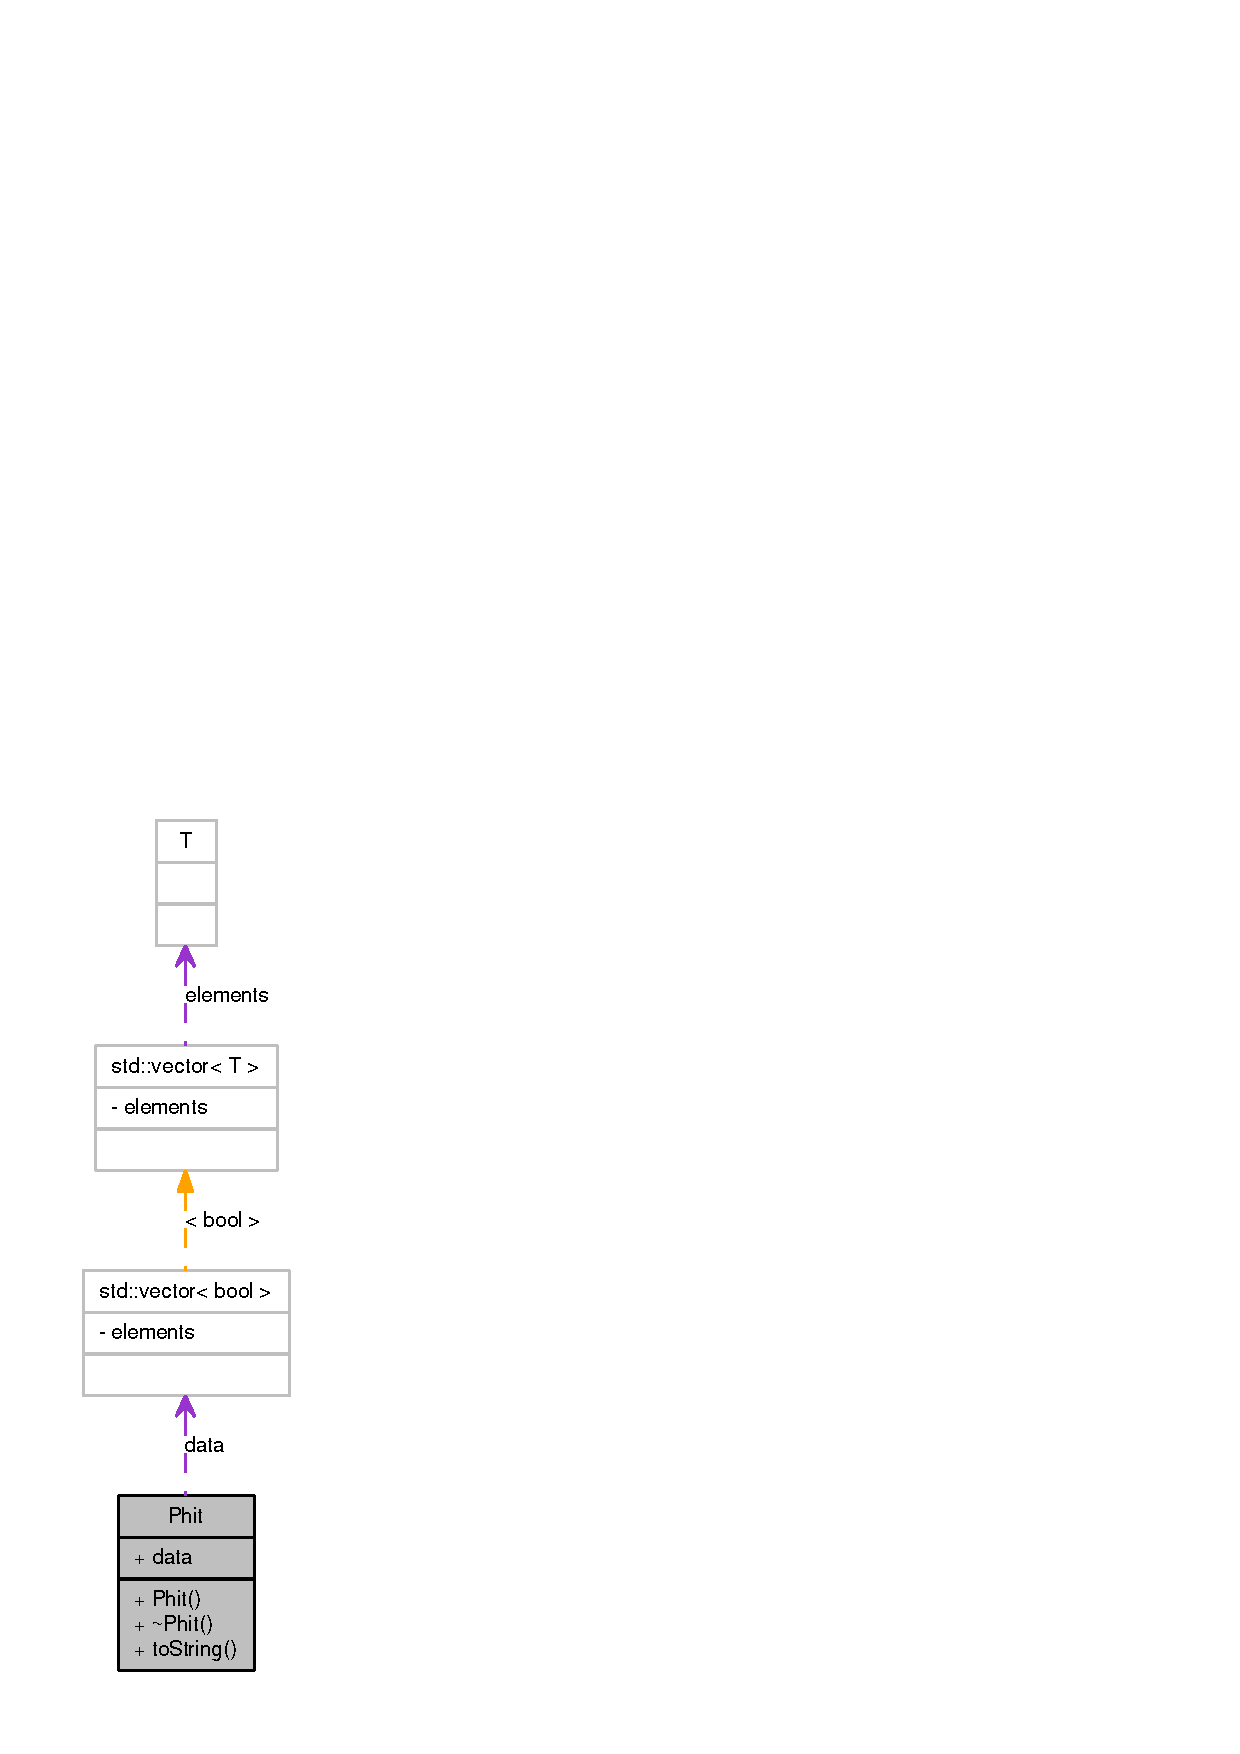
\includegraphics[height=400pt]{classPhit__coll__graph}
\end{center}
\end{figure}
\subsection*{Public Member Functions}
\begin{CompactItemize}
\item 
{\bf Phit} ()
\item 
{\bf $\sim$Phit} ()
\item 
string {\bf toString} () const 
\end{CompactItemize}
\subsection*{Public Attributes}
\begin{CompactItemize}
\item 
vector$<$ bool $>$ {\bf data}
\end{CompactItemize}


\subsection{Detailed Description}


Definition at line 40 of file flit.h.

\subsection{Constructor \& Destructor Documentation}
\index{Phit@{Phit}!Phit@{Phit}}
\index{Phit@{Phit}!Phit@{Phit}}
\subsubsection[{Phit}]{\setlength{\rightskip}{0pt plus 5cm}Phit::Phit ()}\label{classPhit_ffcfc94e38419efe2318add1830fa3cc}




Definition at line 30 of file flit.cc.\index{Phit@{Phit}!$\sim$Phit@{$\sim$Phit}}
\index{$\sim$Phit@{$\sim$Phit}!Phit@{Phit}}
\subsubsection[{$\sim$Phit}]{\setlength{\rightskip}{0pt plus 5cm}Phit::$\sim$Phit ()}\label{classPhit_6901e28fe471c2db1597bb2ce8ac25ba}




Definition at line 34 of file flit.cc.

References data.

\subsection{Member Function Documentation}
\index{Phit@{Phit}!toString@{toString}}
\index{toString@{toString}!Phit@{Phit}}
\subsubsection[{toString}]{\setlength{\rightskip}{0pt plus 5cm}string Phit::toString () const}\label{classPhit_71d43cdc2c23a7788b8724a4b12b261b}




Definition at line 40 of file flit.cc.

References data.

\subsection{Member Data Documentation}
\index{Phit@{Phit}!data@{data}}
\index{data@{data}!Phit@{Phit}}
\subsubsection[{data}]{\setlength{\rightskip}{0pt plus 5cm}vector$<$bool$>$ {\bf Phit::data}}\label{classPhit_de0670c9ef9f280e53ce73980b785a8c}




Definition at line 45 of file flit.h.

Referenced by toString(), and $\sim$Phit().

The documentation for this class was generated from the following files:\begin{CompactItemize}
\item 
{\bf flit.h}\item 
{\bf flit.cc}\end{CompactItemize}
